%%%
% Plantilla de Memoria
% Modificación de una plantilla de Latex de Nicolas Diaz para adaptarla 
% al castellano y a las necesidades de escribir informática y matemática%
% Editada por: Mario Román
%
% License:
% CC BY-NC-SA 3.0 (http://creativecommons.org/licenses/by-nc-sa/3.0/)
%%%

%%%%%%%%%%%%%%%%%%%%%%%%%%%%%%%%%%%%%%%%%
% Thin Sectioned Essay
% LaTeX Template
% Version 1.0 (3/8/13)
%
% This template has been downloaded from:
% http://www.LaTeXTemplates.com
%
% Original Author:
% Nicolas Diaz (nsdiaz@uc.cl) with extensive modifications by:
% Vel (vel@latextemplates.com)
%
% License:
% CC BY-NC-SA 3.0 (http://creativecommons.org/licenses/by-nc-sa/3.0/)
%
%%%%%%%%%%%%%%%%%%%%%%%%%%%%%%%%%%%%%%%%%

%----------------------------------------------------------------------------------------
%	PAQUETES Y CONFIGURACIÓN DEL DOCUMENTO
%----------------------------------------------------------------------------------------

%%% Configuración del papel.
% microtype: Tipografía.
% mathpazo: Usa la fuente Palatino.
\documentclass[a4paper, 20pt, dvipsnames]{article}
\usepackage[a4paper,margin=1in]{geometry}
\usepackage[protrusion=true,expansion=true]{microtype}
\usepackage{mathpazo}

% Indentación de párrafos para Palatino
\setlength{\parindent}{0pt}
  \parskip=8pt
\linespread{1.05} % Change line spacing here, Palatino benefits from a slight increase by default


%%% Castellano.
% noquoting: Permite uso de comillas no españolas.
% lcroman: Permite la enumeración con numerales romanos en minúscula.
% fontenc: Usa la fuente completa para que pueda copiarse correctamente del pdf.
\usepackage[spanish,es-noquoting,es-lcroman,es-tabla,,es-nodecimaldot]{babel}
\usepackage[utf8]{inputenc}
\usepackage{fontenc}
\selectlanguage{spanish}


%%% Gráficos
\usepackage{graphicx} % Required for including pictures
\usepackage{wrapfig} % Allows in-line images
\usepackage[usenames,dvipsnames]{color} % Coloring code
%\usepackage{subcaption}
\usepackage{subfig}
\graphicspath{{./../fig/}}
\captionsetup{width=0.8\textwidth}

%%% Matemáticas
\usepackage{amsmath}
\usepackage{physics} % para las derivadas parciales
\usepackage[Symbol]{upgreek} %pi

%%% Pseudocódigo
\usepackage[htt]{hyphenat} % Permite salto de líneas en texttt
\usepackage{algorithmicx}
\usepackage[ruled]{algorithm}
\usepackage{algpseudocode}

\newcommand{\alg}{\texttt{algorithmicx}}
\newcommand{\old}{\texttt{algorithmic}}
\newcommand{\euk}{Euclid}
\newcommand\ASTART{\bigskip\noindent\begin{minipage}[b]{0.5\linewidth}}
\newcommand\ACONTINUE{\end{minipage}\begin{minipage}[b]{0.5\linewidth}}
\newcommand\AENDSKIP{\end{minipage}\bigskip}
\newcommand\AEND{\end{minipage}}


%%% Tablas
\usepackage{tabularx}
\usepackage{float}
\usepackage{adjustbox}
\usepackage{booktabs}

% Enlaces y colores
\usepackage{hyperref}
\usepackage[dvipsnames]{xcolor}
\definecolor{webgreen}{rgb}{0,0.5,0}
\hypersetup{
  colorlinks=true,
  citecolor=RoyalBlue,
  urlcolor=RoyalBlue,
  linkcolor=RoyalBlue
}

%%% Código
\usepackage{listings}
\lstset{
  basicstyle=\ttfamily,
  columns=fullflexible,
  %frame=single,
  breaklines=true
}

%%% Gráficas
\usepackage{pgfplots}
\pgfplotsset{compat=1.15}

%%% Bibliografía
\usepackage[backend=biber]{biblatex}
\DefineBibliographyStrings{spanish}{
  urlseen = {Accedido}
}
\addbibresource{bibliography.bib}


\newcommand{\training}{\textit{training }}
\newcommand{\test}{\textit{test }}
\newcommand{\RF}{\textit{Random Forest }}

\DeclareMathOperator{\acc}{\texttt{accuracy}}

%%% Subsubsection con letras
\renewcommand{\thesubsubsection}{\thesubsection.\alph{subsubsection}}

%%% Itemize, enumitem
\usepackage{paralist}
\usepackage{enumitem}

\usepackage[section]{placeins}
% \makeatletter
% \AtBeginDocument{%
%   \expandafter\renewcommand\expandafter\subsection\expandafter
%     {\expandafter\@fb@secFB\subsection}%
%   \newcommand\@fb@secFB{\FloatBarrier
%     \gdef\@fb@afterHHook{\@fb@topbarrier \gdef\@fb@afterHHook{}}}%
%   \g@addto@macro\@afterheading{\@fb@afterHHook}%
%   \gdef\@fb@afterHHook{}%
% }
% \makeatother


%%% Entornos personalizados
\newenvironment{bloque}[1]
{
\begin{tabular}{|l|}
 \multicolumn{1}{c}{\textbf{\large #1}} \\
 \hline
 \textbf{Capa/bloque} \\
 \hline}
{
 \\\hline
    \end{tabular}   
}

\newenvironment{modelo}[1]
{
\begin{tabular}{ |p{4cm}||p{1.5cm}|p{1.5cm}|  }
 \multicolumn{3}{c}{\textbf{\large #1}} \\
 \hline
 \textbf{Capa/bloque} & \textbf{Entrada} & \textbf{Salida} \\
 \hline}
{
 \\\hline
    \end{tabular}   
}

%----------------------------------------------------------------------------------------
%	TÍTULO
%----------------------------------------------------------------------------------------
% Configuraciones para el título.
% El título no debe editarse aquí.
\renewcommand{\maketitle}{
  \begin{flushright} % Right align
  
  {\LARGE\@title} % Increase the font size of the title
  
  \vspace{50pt} % Some vertical space between the title and author name
  
  {\large\@author} % Author name
  \\\@date % Date
  \vspace{40pt} % Some vertical space between the author block and abstract
  \end{flushright}
}

%% Título
\title{\textbf{Título}\\ % Title
Subtítulo} % Subtitle

\author{\textsc{Autor1,\\Autor2} % Author
\\{\textit{Universidad de Granada}}} % Institution

\date{\today} % Date

%-----------------------------------------------------------------------------------------
%	DOCUMENTO
%-----------------------------------------------------------------------------------------

\begin{document}

%-----------------------------------------------------------------------------------------
%	TITLE PAGE
%-----------------------------------------------------------------------------------------

\begin{titlepage} % Suppresses displaying the page number on the title page and the subsequent page counts as page 1
	
	\raggedleft % Right align the title page
	
	\rule{1pt}{\textheight} % Vertical line
	\hspace{0.05\textwidth} % Whitespace between the vertical line and title page text
	\parbox[b]{0.8\textwidth}{ % Paragraph box for holding the title page text, adjust the width to move the title page left or right on the page
		
		{\Huge\bfseries Proyecto final:\\[0.5\baselineskip] Generación
                  de \LaTeX{} a partir de imágenes de fórmulas
                  \\[0.5\baselineskip]\\[2\baselineskip]} % Title
		{\large\textit{Curso 2020/21}\\[0.5\baselineskip]Visión por computador\\[1.5\baselineskip] }% Subtitle or further description
		{\Large\textsc{José Antonio Álvarez Ocete, \\Daniel Pozo Escalona}\\[1.5\baselineskip]joseantonioao32@correo.ugr.es,\\danipozo@correo.ugr.es} % Author name, lower case for consistent small caps
		
		\vspace{0.4\textheight} % Whitespace between the title block and the publisher
		
		{\noindent \\[0.5\baselineskip] }\\[\baselineskip] % Publisher and logo
	}

\end{titlepage}

%% Resumen (Descomentar para usarlo)
%\renewcommand{\abstractname}{Resumen} % Uncomment to change the name of the abstract to something else
%\begin{abstract}
% Resumen aquí
%\end{abstract}

%% Palabras clave
%\hspace*{3,6mm}\textit{Keywords:} lorem , ipsum , dolor , sit amet , lectus % Keywords
%\vspace{30pt} % Some vertical space between the abstract and first section

%% Índice
{\parskip=2pt
	\tableofcontents
}
\pagebreak

\newpage

\section{Introducción}

Nuestro objetivo en este trabajo será desarrollar un modelo que, dada una imagen
producida al compilar código \LaTeX{} asociado a una fórmula, prediga el código
\LaTeX{} que fue utilizado para compilarla. La aplicación práctica de un modelo
de estas características permitiría agilizar procesos de digitalización de
documentos matemáticos, o la redacción de los mismos a partir de fuentes de cuyo
código original no se dispone.

Para ello utilizaremos un esquema codificador-decodificador basado en
\emph{transformers} \cite{vaswani2017attention}.


\section{Bases de datos}
\label{sec:datasets}

Las bases de datos para el problema son:

\begin{itemize}
\item
  \textsc{im2latex-100k} \cite{kanervisto_anssi_2016_56198}, y
\item
  \textsc{imlatex-170k} \cite{im2latex_170k}: contiene 65000 ejemplos, que se
  añaden a los 100000 de im2latex-100k.
\end{itemize}
% TODO: revisar que (todas) las referencias están bien puestas.

Una muestra de \textsc{imlatex-170k} se puede ver en la figura
\ref{fig:muestras-1}.

Ambas bases de datos contienen ambigüedad en los ejemplos, en forma de fórmulas
o segmentos de fórmulas que, escritos de distinta forma, producen la misma
imagen. Dedicaremos parte del tiempo del proyecto a diseñar formas de normalizar
estos datos, para mejorar los resultados. Entraremos en detalle más adelante.

Debido a esta ambigüedad, las evaluaciones iniciales con modelos de referencia y
las finales pueden no ser directamente comparables. Esto lo paliaremos de dos
formas: con la base de datos sintética que introducimos a continuación, y
evaluando los modelos de referencia en la base de datos normalizada. Además, hay
que tener en cuenta que lo relevante en este problema es dar expresiones
\LaTeX{} que produzcan las imágenes que se proporcionen al modelo, más que estas
coincidan con unas prefijadas.

En la práctica, utilizaremos únicamente \textsc{im2latex-170k}, ya que contiene
a la anterior.

\begin{figure}[H]
	\centering
	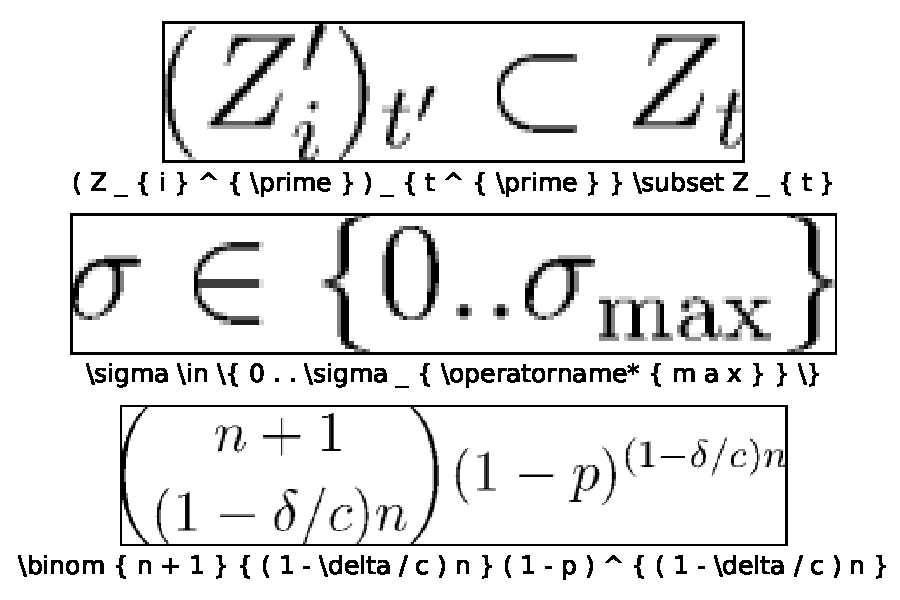
\includegraphics{./fig/ejemplo-im2latex.pdf}
	\caption{Tres muestras de im2latex-170k.}
	\label{fig:muestras-1}
\end{figure}


\subsection{Base de datos sintética: Toy}
\label{sec:toy}

Lo primero que hemos hecho ha sido crear una base de datos similar a las que
pretendemos tratar, en la que las fórmulas han sido generadas a partir de una
gramática relativamente sencilla, que contiene una cantidad pequeña de símbolos.
A esta base de datos la hemos denominado \textbf{Toy}.

Hemos generado 50.000 ejemplos distintos. Los guiones Python que hemos escrito a
tal efecto permiten cambiar la gramática y generar conjuntos de datos con
cantidades arbitrarias de ejemplos únicos.

Además, esta base de datos puede ser útil para evaluar cambios a la arquitectura
o hiperparámetros de forma menos costosa.

\begin{figure}[H]
	\centering
	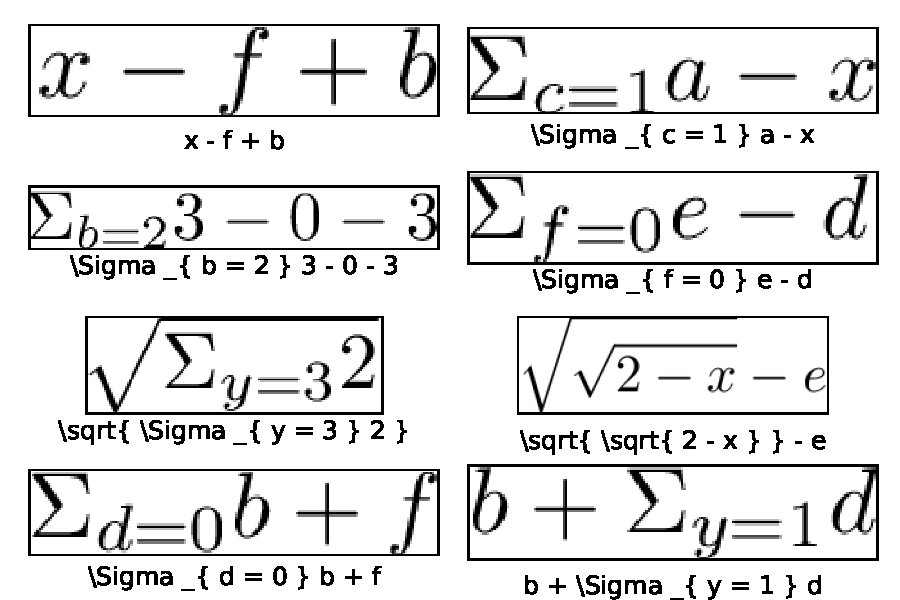
\includegraphics{fig/ejemplo-sintetica.pdf}
	\caption{Muestras de la base de datos sintética.}
	\label{fig:muestras-sintetica}
\end{figure}


\section{Modelo propuesto}
\label{sec:model}

El modelo que proponemos es el siguiente:

\begin{itemize}
\item
  Un codificador, formado por una red convolucional, seguido por un modelo
  \emph{transformer}.

\item
  Un decodificador \emph{transformer}, que emplea atención multi-cabezal sobre
  la salida del codificador y sobre una secuencia potencialmente incompleta,
  para predecir el siguiente token de la fórmula. Es decir, es un modelo de
  lenguaje condicional que modela $p(x_t | V, x_1, ..., x_{t-1})$, donde $V$ es
  la salida del codificador.
\end{itemize}

Utilizaremos una red convolucional para obtener las características de las
imágenes de entrada. Este vector de características será la entrada para el
modelo codificador-decodificador.

Aunque posteriormente el modelo de referencia que se presenta a continuación
sufrirá ciertas variaciones, el esquema general no variará. Este modelo posee un
codificador convolucional con tres capas Conv-BN-ELU-MaxPooling y una sola capa
de atención en el codificador y en el decodificador.

% TODO: quitar esta proxima linea, que hace que no salga el modelo.
% \iffalse
\begin{figure}[h]
	\centering
	
	\subfloat{
		\begin{bloque}{Codificador convolucional}
			Conv2D-BN-ELU(64 filtros) \\
			MaxPooling2D(2$\times$2) \\
			Conv2D-BN-ELU(64 filtros) \\
			MaxPooling2D(2$\times$2) \\
			Conv2D-BN-ELU(64 filtros) \\
			MaxPooling2D(2$\times$2)
		\end{bloque}
	}
	\subfloat{
		\begin{bloque}{Codificador \textit{transformer}}
			Codif. conv. \\
			Codificación de posición \\
			Dropout \\
			Capa de codificador
		\end{bloque}
	}
	\subfloat{
		\begin{bloque}{Decodificador \textit{transformer}}
			Embedding \\
			Codificación de posición \\
			Dropout \\
			Capa de decodificador
		\end{bloque}
	}
	
	\caption{Bloques del modelo de referencia.}
	\label{fig:bloques-referencia}
\end{figure}
% \fi


\section{Detalles técnicos y de implementación}

En esta sección detallamos algunas cuestiones que pueden tener relevancia de
cara a reproducir el trabajo realizado y entender las dificultades técnicas que
hemos afrontado.

\subsection{\emph{Hardware} empleado}

Para los experimentos, hemos empleado máquinas con las siguientes
características:
\begin{itemize}
\item
  30 GB RAM,
\item
  procesadores de 8 núcleos, modelo no especificado,
\item
  GPU Nvidia Quadro P5000 o P6000.
\end{itemize}

\subsection{Arquitectura y configuración de experimentos}

El código de los experimentos ha sido concebido de la siguiente forma: como un
guion Python principal, que se encarga de leer los datos, configurar el modelo,
entrenarlo y guardar los resultados. La configuración del modelo depende de una
serie de banderas de línea de órdenes que el programa interpreta. Esto nos ha
permitido lanzar múltiples experimentos en paralelo, sin necesidad de modificar
el código. El código se encuentra disponible en
\url{https://github.com/Ocete/LaTeXrec}.

\subsection{Preprocesamiento de datos}

Para las imágenes, el procesamiento que realizamos es redimensionarlas a una
altura común, manteniendo la relación de aspecto. Tras esto, eliminamos los
ejemplos con imágenes demasiado grandes para ser procesadas por el modelo,
debido al coste cuadrático del mecanismo de atención.

Para las fórmulas, utilizamos el \emph{tokenizer} de TensorFlow \cite{tokenizer}
para obtener el alfabeto de entrada. Por lo tanto, este no es fijo sino que
depende del conjunto de datos. Esto nos permite codificar las fórmulas
numéricamente.

\subsection{Guardado de modelos}

TensorFlow proporciona algunas utilidades para guardar modelos y cargarlos
posteriormente, lo que permite entrenarlos en varias fases, guardar los modelos
en varios puntos del entrenamiento o usarlos para obtener predicciones después
de entrenados.

Sin embargo, no hemos conseguido que funcionen con nuestro modelo, que es
relativamente complejo, en el sentido de que ha sido creado mediante \emph{model
  subclassing} y toma varios argumentos que no son entradas (las máscaras) al
ser llamado.

Esto es un obstáculo que habría de ser solventado de cara a una posible
aplicación del modelo.

\subsection{Lectura eficiente}

Una vez comenzamos a trabajar con la base de datos \textsc{im2latex-170K}
descubrimos que esta no cabía por completo en memoria. De hecho, no cabía ni una
cuarta parte. De cara a implementar una solución escalable y eficiente a este
problema creamos una clase, \texttt{LaTeXrecDataset}, que hereda de
\texttt{tf.data.Dataset} \cite{tf_dataset}, de TensorFlow. Esta clase nos
permite leer las imágenes conforme el modelo las necesita y, al mismo tiempo,
eliminarlas de memoria cuando dejan de hacerlo. Todo esto se procesa de forma
automática y muy cómodamente, además de permitirnos implementar
\emph{prefetching}. Esto es, lectura anticipada de los datos antes de que hagan
falta para acelerar el proceso.

\subsection{\emph{Early Stopping}}
\label{early-stopping}

Hemos implementado \emph{early stopping} con el objetivo de reducir el tiempo
de cómputo de algunos experimentos cuando se estanca su evolución. Esta
implementación ha sido manual ya que el entrenamiento de los modelos se
realiza paso a paso manualmente y no podemos utilizar el \emph{callbacks}
de Tensorflow. Dicho \emph{early stopping} esta basado la precisión en
validación, no en la pérdida.

\subsection{Registros (\emph{logs})}

Añadimos un sistema de \emph{logging} a distintos archivos y a la salida
estándar, para facilitar la depuración de errores y el seguimiento del progreso
del programa.


\section{Características añadidas al modelo}

En esta sección describimos las distintas características implementadas sobre el
modelo inicial descrito con anterioridad. Los resultados de las mismas se
describen en la sección de experimentos.


\subsection{Eliminación de ambigüedades}
\label{feature:rem-amb}

Como ya discutimos en la sección \ref{sec:datasets}, en este problema
encontramos ambigüedad en la salida de los datos. Distintas expresiones \LaTeX{}
generan la misma salida o una casi indistinguible en la imagen. Por ejemplo,
\emph{\textbackslash sin} y \emph{\textbackslash operatorname\{sin\}}: $\sin(x)$
frente a $\operatorname{sin}(x)$.

Esto hace que el aprendizaje sea más difícil. El primer cambio que hicimos tras
tener un modelo funcional fue eliminar este tipo de ambigüedades en los
datos. Cabe aclarar que aunque estemos alterando los datos, la imagen \LaTeX{}
obtenida es exactamente la misma en todos estos casos.

Utilizamos el \emph{tokenizer} de TensorFlow \cite{tokenizer} para generar una
lista de tokens de las primeras 60.000 imágenes en la que basarnos. Estudiando
esta lista hemos decidido modificar las siguientes ambigüedades, buscando un
balance entre implementación sencilla y que merezca la pena porque sean lo
suficientemente relevantes:

\begin{itemize}
\item
  Los operadores con nombre más famosos (como seno y máximo), tienen un
  comando particular en \LaTeX{}: \emph{\textbackslash sin}, y
  \emph{\textbackslash max}. Utilizaremos estos comandos en vez de los
  respectivo \emph{\textbackslash operatorname\{sin\}} y \emph{\textbackslash
    operatorname\{max\}}, siempre que se pueda. Aplicaremos esta misma
  sustitución para los comandos con un asterisco: \emph{\textbackslash
    operatorname* \{sin\}}. La lista completa de operadores a la que le
  aplicamos essta sustitución es la siguiente: `\emph{\textbackslash sin},
  \emph{\textbackslash cos}, \emph{\textbackslash tan}, \emph{\textbackslash
    arcsin}, \emph{\textbackslash arccos}, \emph{\textbackslash arctan},
  \emph{\textbackslash sinh}, \emph{\textbackslash cosh}, \emph{\textbackslash
    tanh}, \emph{\textbackslash max}, \emph{\textbackslash min},
  \emph{\textbackslash exp}, \emph{\textbackslash log}, \emph{\textbackslash
    ln}, \emph{\textbackslash sup}, \emph{\textbackslash inf},
  \emph{\textbackslash lim}, \emph{\textbackslash dim}, \emph{\textbackslash
    deg}, \emph{\textbackslash ker}, \emph{\textbackslash cot},
  \emph{\textbackslash Pr}, \emph{\textbackslash lg}, \emph{\textbackslash arg},
  \emph{\textbackslash det}, \emph{\textbackslash vol}.

\item
  El comando \emph{\textbackslash prime} se utiliza en \LaTeX{} para mostrar
  una comilla grande. En caso de utilizarse como exponente (\emph{
    \textbackslash \textasciicircum \{ \textbackslash prime \}}) tiene la misma
  representación gráfica que una comilla simple: \textbf{'}. Sustituiremos la
  expresión: `\emph{ \textbackslash \textasciicircum \{ \textbackslash prime
    \}}` por '.

\item
  Los símbolos de llaves `\{` y `\}` se pueden escribir también como `\emph{
    \textbackslash brace }` y `\emph{ \textbackslash rbrace }`
  respectivamente. Los sustituiremos por la versión más corta que es, además,
  más general ya que se puede utilizar tanto en modo texto como en modo
  matemáticas.

\item
  El símbolo de la daga se puede escribir en $LaTex$ utilizando tanto `\emph{
    \textbackslash dagger }` como `\emph{ \textbackslash dag }`. Aunque este
  símbolo apenas aparece en nuestras fórmulas, añadir esta sustitución es una
  línea extra que no añade complejidad ninguna. Utilizaremos su versión más
  corta.

\item
  Finalmente, la tipografía aplicada al utilizar `\emph{\textbackslash cal}`
  y `\emph{\textbackslash mathcal}` es exactamente la misma aunque su sintaxis
  es distinta. `\emph{\textbackslash cal}` se utiliza para palabras o letras
  sueltas: `\emph{\textbackslash prime} A`; mientras que `\emph{\textbackslash
    mathcal}` se utiliza para expresiones más complejas: `\emph{\textbackslash
    mathcal} \{ sin \textasciicircum \{ 2 \} ( x ) \}`. Puesto que el uso de
  `\emph{\textbackslash cal}` está obsoleto y `\emph{\textbackslash mathcal}` es
  más general, utilizaremos este último, reajustando la sintaxis conforme sea
  necesario.
\end{itemize}

\subsection{Atención eficiente}
\label{feature:fast-att}

Uno de los principales escollos que hemos encontrado ya desde el trabajo
preliminar en este proyecto es el enorme consumo de memoria del modelo
\emph{transformer}. Esto se debe a que, en cada capa de atención, se ha de
calcular la matriz de atención, de tamaño cuadrático en la longitud de la
secuencia procesada. En el caso de las características provenientes de la
imagen, esta secuencia puede alcanzar longitud 500.

Recientemente, se han propuesto múltiples alternativas para aproximar el
mecanismo de atención de forma más eficiente \cite{tay2020efficient}. En la
tabla 1 de este artículo de revisión se encuentran listadas todas las
alternativas, junto con algunas características de las mismas.

Hemos seleccionado, de entre las que permiten emplear un decodificador, la
atención rápida mediante el mecanismo FAVOR+
\cite{choromanski_rethinking_2020}. Hemos adaptado la implementación de los
autores
(\url{https://github.com/google-research/google-research/tree/master/performer/fast_attention/tensorflow})
y la hemos probado en algunos experimentos.

Esta técnica se basa en emplear características aleatorias de Fourier \cite{rff}
para aproximar la función Softmax, de forma que en la ecuación de la atención
\[
  \text{Attn}(Q, K, V) = \text{Softmax}(QK^{T})V
\]
se pueden reemplazar las matrices $Q$ y $K$ por matrices $Q'$ y $K'$ con una
dimensión independiente del tamaño de la secuencia a procesar, y tales que
$Q'K'^{T}$ aproxima a $\text{Softmax}(QK^{T})$. Así se pueden reordenar los
cálculos, evitando la complejidad cuadrática.


\subsection{Codificación posicional 2-dimensional}
\label{feature:cod-pos-2d}

La capa de \emph{self attention}, en la que se basan los bloques
\textit{transformer}, sigue un modelo de conexión ``todos con todos'', por lo
que pierde la información posicional de los elementos que recibe. Es por ello
que se añade codificación posicional, para añadir artificialmente dicha
información de la posición de cada palabra.

Sin embargo, la codificación posicional usual está pensada para dar información
acerca de las posiciones relativas de distintos elementos en una secuencia
plana, como puede ser un texto. En el caso de imágenes, esto supone una pérdida
de información.

Para paliar esta pérdida de información hemos implementado codificación
posicional 2-dimensional, utilizando así la información relativa de las
características al completo.

En nuestro caso particular, añadimos esa codificación posicional a la salida de
nuestra red convolucional con las características de la imagen obtenidas.

La implementación de la codificación posicional 2-dimensional ha sido traducida
a partir de la disponible
\href{https://github.com/wzlxjtu/PositionalEncoding2D/blob/master/positionalembedding2d.py}{en
  este fichero}.

\subsection{Métrica BLEU}

Hacia el final del desarrollo hemos implementado la
\href{https://en.wikipedia.org/wiki/BLEU}{métrica BLEU} para evaluar de forma
más intuitiva los resultados obtenidos. Esta métrica nos da una estimación de
cuanto se parecen dos cadenas de tokens. Suele utilizarse para comparar cuán
buena es una traducción de lenguaje a otro, y la utilizaremos en el último
experimento.

% Referencia: [tensor2tensor](https://github.com/tensorflow/tensor2tensor/blob/master/tensor2tensor/utils/bleu\_hook.py#L132).

\section{Parámetros del modelo}
\label{sec:params}

% TODO: aqui explicamos los parámetros del modelo basico

\section{Experimentos}

\subsection{Metodología}

Realizaremos experimentos sobre las dos bases de datos de las que disponemos: la
sintética e \textsc{im2latex-170k}. Para la sintética, los experimentos tienen
el objetivo principal de comprobar si algunas de las características
implementadas tienen verdadera utilidad o no. Para comprobar su efectividad nos
bastará con dividir el conjunto de datos en entrenamiento y validación con una
proporción del 90\% / 10\%.

Sin embargo, con la base de datos \textsc{im2latex-170k} buscamos también poner
a prueba el modelo. Para ello dividiremos el modelo en entrenamiento frente a
test con proporción 90\% / 10\%. Este subconjunto de test es apartado antes de
realizar ningún experimento.

A continuación para cada experimento el conjunto de entrenamiento se baraja y se
vuelve a dividir en entrenamiento y validación con proporción 90\% / 10\%. De
esta forma, el subconjunto de validación varía aleatoriamente entre
experimentos.

\subsection{Experimentos sobre los datos sintéticos}

En esta primera sección detallamos algunos de los experimentos más interesantes
realizados sobre la base de datos sintética \ref{sec:toy}. Vamos a destacar 3:
uno inicial sobre el modelo sin alteraciones que servirá como referencia para
los demás, y otros dos que prueban algunas de las modificaciones implementadas.

\subsubsection{Experimento inicial sobre los datos sintéticos}
\label{exp:toy1}

Para el primer experimento nos ceñimos al modelo propuesto \ref{sec:model} junto
con los parámetros especificados \ref{sec:sec:params} sin ninguna
modificación. Los resultados obtenidos han sido los siguientes:

\begin{table}[H]
	\centering
	\begin{tabular}{llllll}
		& Precisión & Precisión en validación & Pérdida & Pérdida en validación & Tiempo (h) \\ \cline{2-6} 
		CNN simple & 0.9201    & 0.5098                  & 0.2242  & 2.8680                & 1.27      
	\end{tabular}
\end{table}

\begin{figure}[H]
	\centering
	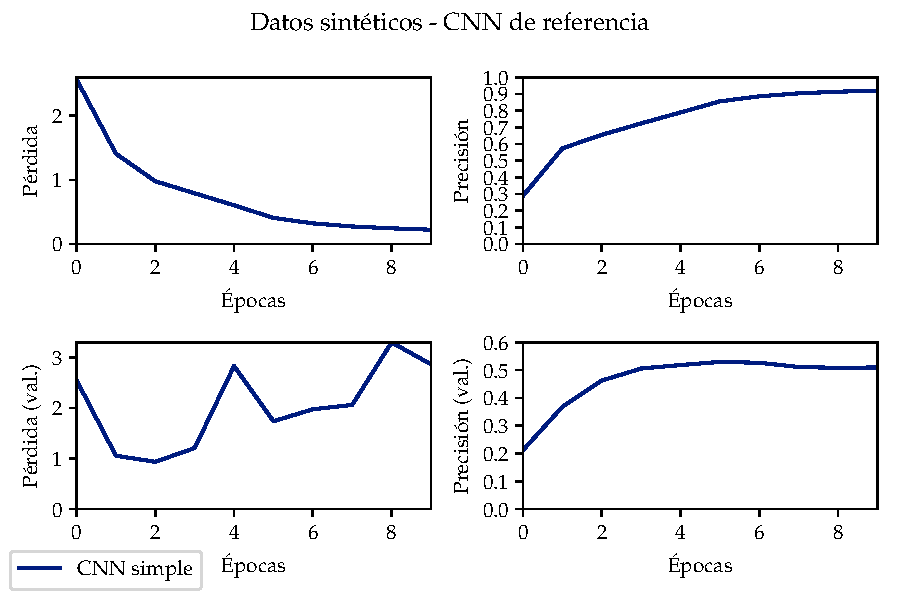
\includegraphics{fig/toy-1.pdf}
\end{figure}

Obtenemos una precisión en entrenamiento del 92.01 \% frente a 50.98 \% en
validación, produciéndose un tremendo sobreajuste sobre los datos de
entrenamiento. En las gráficas vemos como 4 o 5 épocas eran suficientes para
ajustar el modelo a los datos. A partir de ese punto, la precisión en validación
baja ligeramente mientras que en entrenamiento continúa subiendo. De la misma
forma, la pérdida acaba subiendo conforme aumenta el número de épocas.

El tiempo de ejecución completo ha sido de 1.27 horas. No es particularmente
alto, pero si consideramos que aún no hemos añadido ningún extra al modelo, y
que la bases de datos utilizada es la sintética, esto nos hace pensar que el
tiempo de ejecuciones de los posteriores experimentos será notablemente alto.

Ese 50.98 \% de precisión en validación nos indica que el modelo acierta el
siguiente símbolo \LaTeX{} esperado en el 50.98 \%, en media, de los casos.


\subsubsection{ResNet}
\label{exp:toy2}

En este segundo experimento cambiamos la red convolucional utilizada para
extraer las características de las imágenes por una ResNet. Mantenemos el resto
de parámetros invariantes para comparar unicamente el resultado de
ResNet. Veamos los resultados obtenidos:

\begin{table}[H]
	\centering
	\begin{tabular}{llllll}
		& Precisión       & Precisión en validación & Pérdida         & Pérdida en validación & Tiempo (h) \\ \cline{2-6} 
		CNN Simple & 0.9201          & 0.5098                  & 0.2242          & 2.8680                & 1.27       \\
		ResNet     & \textbf{0.9340} & \textbf{0.5320}         & \textbf{0.1922} & \textbf{1.4217}       & 1.40      
	\end{tabular}
\end{table}

\begin{figure}[H]
	\centering
	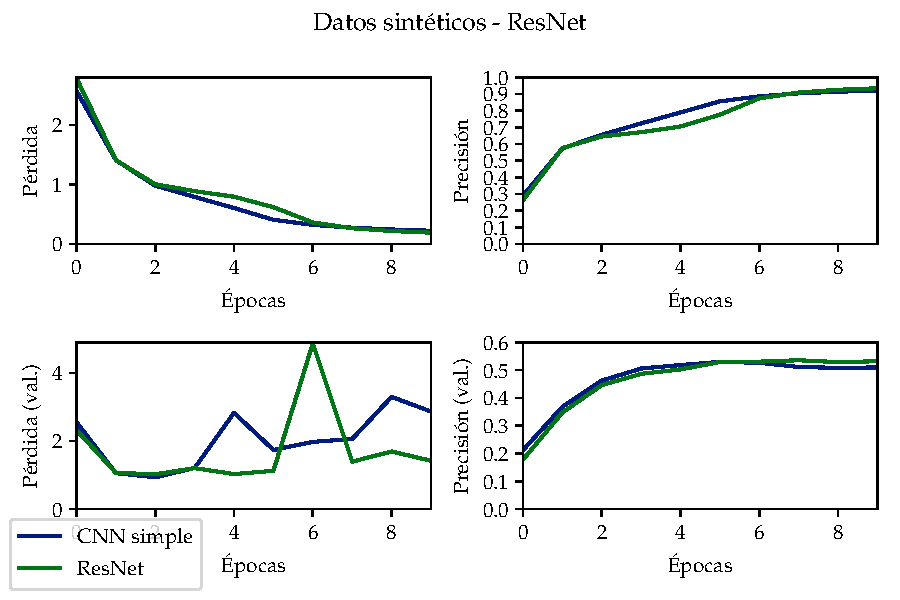
\includegraphics{fig/toy-2.pdf}
\end{figure}

Vemos como el modelo mejora en todas las métricas estudiadas. Si bien el modelo
con ResNet tarda un poco más en ajustarse a los datos, como se aprecia en la
gráfica de precisión en validación, también se sobreajusta menos a los mismos -
o al menos tarda más en hacerlo. A pesar de que la mejora en un 3\% de precisión
no demasiado remarcable, si que nos indica cierta mejora así que nos incita a
probar esta misma comparación en la base de datos Im2Latex, como se realiza en
el experimento \ref{exp:3b}.

En cuanto al tiempo, este aumenta ligeramente, lo que se traducirá en una
posterior sobrecarga temporal en su aplicación sobre \textsc{im2latex-170k}.


\subsubsection{Atención rápida}
\label{exp:toy3}

En este tercer y último experimento sobre los datos sintéticos probamos la
atención eficiente explicada en la sección \ref{feature:fast-att}. Volvemos a
utilizar la red convolucional simple y mantenemos los mismos parámetros. Veamos
los resultados obtenidos:

\begin{table}[h]
	\centering
	\begin{tabular}{llllll}
		& Precisión       & Precisión en validación & Pérdida         & Pérdida en validación & Tiempo (h) \\ \cline{2-6} 
		CNN Simple         & 0.9201          & 0.5098                  & 0.2242          & 2.8680                & 1.27       \\
		ResNet             & 0.9340          & \textbf{0.5320}         & 0.1922          & \textbf{1.4217}       & 1.40       \\
		Atención eficiente & \textbf{0.9411} & 0.4936                  & \textbf{0.1652} & 1.5576                & 1.29      
	\end{tabular}
\end{table}

\begin{figure}[H]
	\centering
	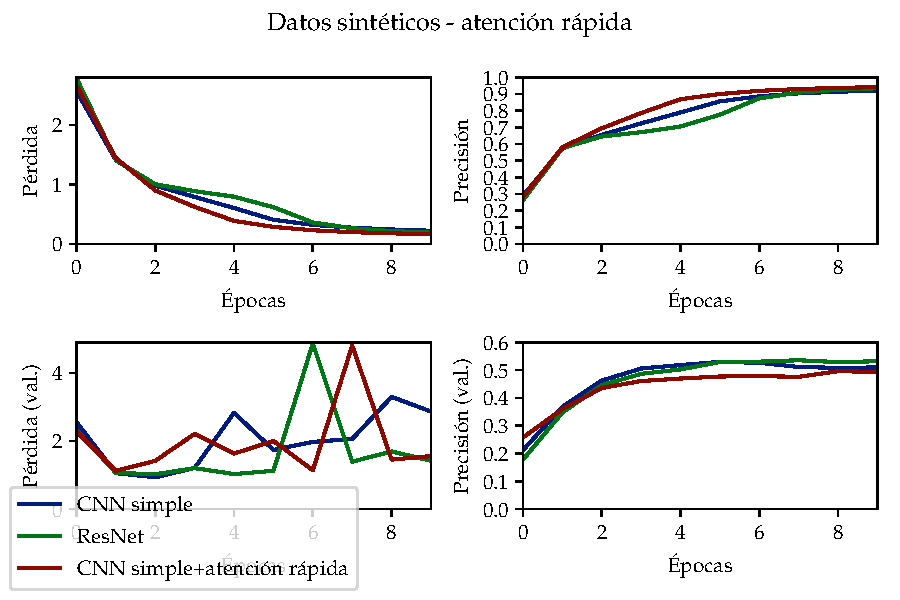
\includegraphics{fig/toy-3.pdf}
\end{figure}
<<<<<<< HEAD
e
Vemos en la tabla como el modelo empeora en precisiñón en validación respecto al experimento original. Como ya explicamos en la sección \ref{feature:fast-att} donde se explica la atención eficiente, el objetivo de ésta es reducir el consumo de memoria, uno de los principales cuellos de botella del modelo. Si bien esto no se percibe particularme ahora ya que el tiempo es practicamente el mismo, nos permitirá aumentar el tamaño del batch estudiado para Im2Latex, como veremos en el experimento \ref{exp:3a}.
=======

Vemos en la tabla como el modelo empeora en precisión en validación respecto al
experimento original. Como ya explicamos en la sección \ref{feature:fast-att}
donde se explica la atención eficiente, el objetivo de esta es reducir el
consumo de memoria, uno de los principales cuellos de botella del modelo. Si
bien esto no se percibe particularmente ahora ya que el tiempo es practicamente
el mismo, nos permitirá aumentar el tamaño del batch estudiado para
\textsc{im2latex-170k}, como veremos en el experimento \ref{exp:3a}.


\subsection{Experimentos sobre \textsc{im2latex-170k}}

Para esta tanda de experimentos ponemos en uso el \emph{early stopping} \ref{early-stopping} implementado anteriormente. Este se dará si no se 
ha mejorado la precisión en validación en un 1\% durante 10 evaluaciones
consecutivas. Realizamos una evaluación cada 50 batches de 32 imágenes
cada uno.

Cabe destacar que estamos utilizando la precisión en validación. Esto es porque nuestro
\emph{early stopping} no busca evitar el sobreajuste sino simplemente reducir el
monumental tiempo de ejecución sobre Im2Latex. De hecho, como veremos, el sobreajuste en
Im2Latex no es ni mucho menos tan relevante como lo es sobre Toy.

\subsubsection{Experimento inicial sobre \textsc{im2latex-170k}}
\label{exp:1}

Para este primer experimento sobre la base de datos \textsc{im2latex-170k}
volvemos al modelo propuesto originalmente \ref{sec:model} junto con los
parámetros comentados \ref{sec:sec:params}, sin modificaciones adicionales. Los
resultados obtenidos han sido los siguientes:

\begin{table}[H]
	\centering
	\begin{tabular}{llllll}
		& Precisión & Precisión en validación & Pérdida & Pérdida en validación & Tiempo (h) \\ \cline{2-6} 
		CNN Simple & 0.8695    & 0.8190                  & 0.6340  & 0.9014                & 8.33      
	\end{tabular}
\end{table}

\begin{figure}[H]
	\centering
	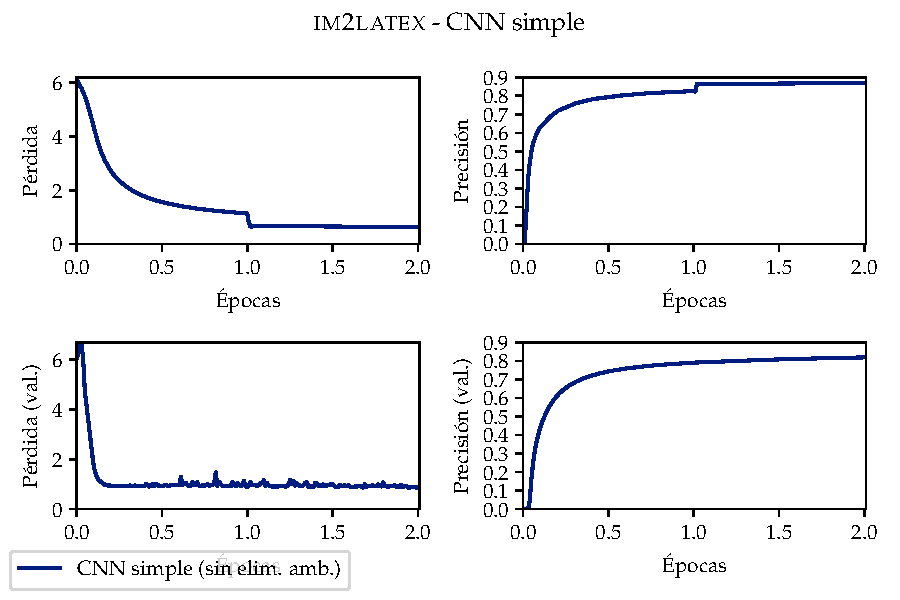
\includegraphics{fig/im2latex-1.pdf}
\end{figure}

Lo primero que observamos tras este experimento fue sin duda el alto valor de
precisión en validación: 81.90 \%. Este valor tiene aún más relevancia si lo
comparamos con el valor obtenido en el experimento \ref{exp:toy1} de un 50.98
\%. Cabría esperar que ante el aumento de complejidad de la gramática estudiada
y las imágenes obtenidas el rendimiento del modelo fuese considerablemente
inferior. Sin embargo, el resultado es exactamente el contrario. Podríamos
pensar que puede deberse a que ante una gramática tan sencilla como la de Toy se
produzca un tremendo sobreajuste. Aunque esto ocurre, no es la causa de su pobre
valor de precisión, como ya se vió en su correspondiente análisis
\ref{exp:toy1}.

Nuestra teoría actual se basa en que el modelo aprende mucho mejor ante tal
cantidad y variedad de imágenes como presenta \textsc{im2latex-170k}. Esto nos
sugiere probar técnicas para aumentar el conjunto de datos. Sin embargo, no nos
valdría con simplemente tomar subimágenes de los datos existentes ya las
imágenes generados por \LaTeX{} se ajustan al texto en ellas, y el tomar
subimágenes invalidaría el resultado esperado.

Volvamos a los resultados del experimento. Como podemos ver en las gráficas, en
este experimento hemos entrenado únicamente durante dos épocas. Esto ya nos
lleva a un tiempo de 8.33 horas, por lo que no era posible realizar más. Hemos
decidido evaluar el modelo entre épocas para tener datos más explicativos, ya
que unicamente dos medidas no nos permitían obtener suficiente información.

Fijándonos en la tabla podemos apreciar como vuelve a producirse sobreajuste:
86.95\% de precisión en entrenamiento frente a 81.90 \% en validación. Sin
embargo, este margen en considerablemente menor que el del 40 \% que se producía
sobre la base de datos sintética.

Cabe destacar la repentina mejora en precisión durante el entrenamiento al
terminar la primera época. Esto nos muestra como el modelo recuerda
especialmente bien los datos proporcionados y puede indicar que entrenar sobre
los mismo datos durante demasiadas épocas podría ser contraproducente. Como
podemos ver en precisión en validación, 2 épocas no son suficientes para
sobreajustarnos a los datos ya que el modelo sigue mejorando hasta el final.

\subsubsection{Eliminar ambigüedades}
\label{exp:2}

En este segundo experimento añadimos la eliminación de ambigüedades explicada en
la sección \ref{feature:rem-amb} a los datos de Im2Latex. Este experimento no se
realizó sobre Toy porque la gramática que definimos para generar dichos datos
carece de ambigüedades.

Mantenemos el resto del modelo y parámetros invariantes. Veamos los resultados obtenidos:

\begin{table}[H]
	\begin{tabular}{llllll}
		\centering
		& Precisión & Precisión en validación & Pérdida & Pérdida en validación & Tiempo (h) \\ \cline{2-6} 
		CNN Simple       & 0.8695    & 0.8190                  & 0.6340  & 0.9014                & 8.33       \\
		CNN Elim. amb. & 0.8701    & 0.8295                  & 0.6272  & 0.8406                & 8.77      
	\end{tabular}
\end{table}

\begin{figure}[H]
	\centering
	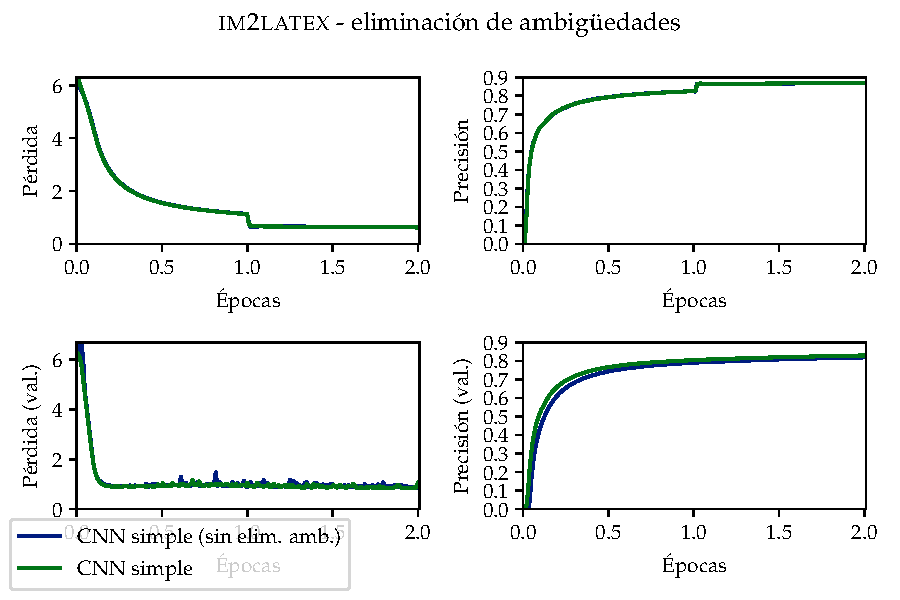
\includegraphics{fig/im2latex-2.pdf}
\end{figure}

Ya que el modelo apenas varía, los resultados son muy parecidos. Mejoramos la
precisión tanto en validación como en entrenamiento, por lo que el preprocesamiento
ha merecido la pena. Adicionalmente, la convergencia del modelo un poco más rápida,
como se aprecia en la gráfica de precisión en validación.

Respecto al tiempo, si bien este aumenta debido al preprocesamiento de los datos,
almacenamos la formulas ya procesadas en un JSON para mitigar dicha sobrecarga de
cara a proximos experimentos. Bastará con leer dicho JSON en vez de realizar de
nuevo el preprocesamiento.

Finalmente, ya que este preprocesamiento aumenta la precisión sin añadir tiempo de
cómputo al modelo, merece la pena en todos los casos. Es por ello que a partir de
ahora todos los experimentos se realizarán sobre los datos sin ambigüedades.

\subsubsection{Atención eficiente}
\label{exp:3a}

Comprobamos ahora la eficacia de la mejora de atención eficiente \ref{feature:fast-att} aplicada sobre la base de datos Im2Latex. Como vimos en el experimento \ref{exp:toy1}, la atención eficiente no tiene como objetivo mejorar la precisión del modelo, sino reducir el uso de memoria y, potencialmente, reducir el tiempo de ejecución del mismo.

Utilizamos para este el modelo anterior, con eliminación de ambigüedades, añadiendole el uso de atención eficiente. Veamos los resultados obtenidos:

\begin{table}[H]
	\centering
	\begin{tabular}{llllll}
		& Precisión       & Precisión en validación & Pérdida         & Pérdida en validación & Tiempo (h)    \\ \cline{2-6} 
		CNN Elim. Amb.  & 0.8701          & \textbf{0.8295}         & \textbf{0.6272} & \textbf{0.8406}       & 8.77          \\
		CNN Aten. Efic. & \textbf{0.8731} & 0.8092                  & 0.6281          & 0.9400                & \textbf{4.68}
	\end{tabular}
\end{table}

\begin{figure}[H]
	\centering
	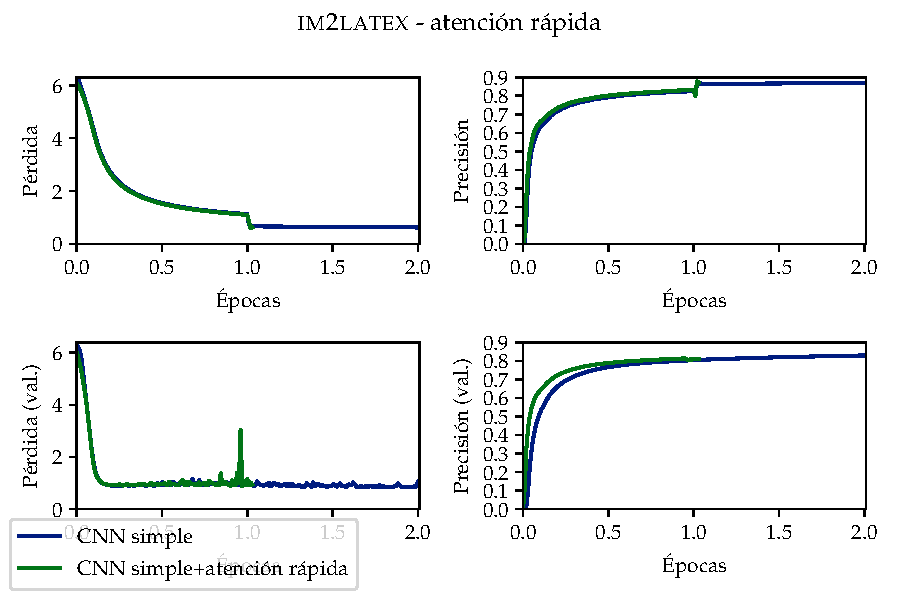
\includegraphics{fig/im2latex-3a.pdf}
\end{figure}

% TODO: creo que el siguiente parrafo esta un poco cogido con pinzaas porque ResNet hace exactamente lo contrario y tambien lo tengo que justificar xd

En este experimento se activo el \emph{early stopping} tras dos evaluacines (100 batches
de 32 imágenes cada uno) de la segunda epoch. Observando la tabla vemos como este modelo empeora
la precisión en validación en un 2\%. Sin embargo, aumenta considerablemente la velocidad
de convergencia. Es por ello que se reduce el tiempo de ejecución total en más de 4 horas.

Si bien se podría estar dando convergencia prematura, evitando que el modelo siga mejorando
a partir de la segunda epoch, veremos en futuros experimentos que este efecto no se produce.

\subsubsection{ResNet}
\label{exp:3b}

Procedemos a estudiar el uso de ResNet en vez de la CNN simple utilizada hasta ahora,
de igual manera que se hizo en el experimento \ref{exp:toy2}. Desactivamos para ello
la atención eficiente del experimento anterior pero mantenemos la eliminación de
ambigüedades. Veamos los resultados obtenidos:

\begin{table}[H]
	\centering
	\begin{tabular}{llllll}
		& Precisión       & Precisión en validación & Pérdida         & Pérdida en validación & Tiempo (h)    \\ \cline{2-6} 
		CNN Elim. Amb.    & \textbf{0.8701} & \textbf{0.8295}         & \textbf{0.6272} & \textbf{0.8406}       & 8.77          \\
		ResNet Elim. Amb. & 0.8674          & 0.8246                  & 0.6412          & 0.8908                & \textbf{8.57}
	\end{tabular}
\end{table}

\begin{figure}[H]
	\centering
	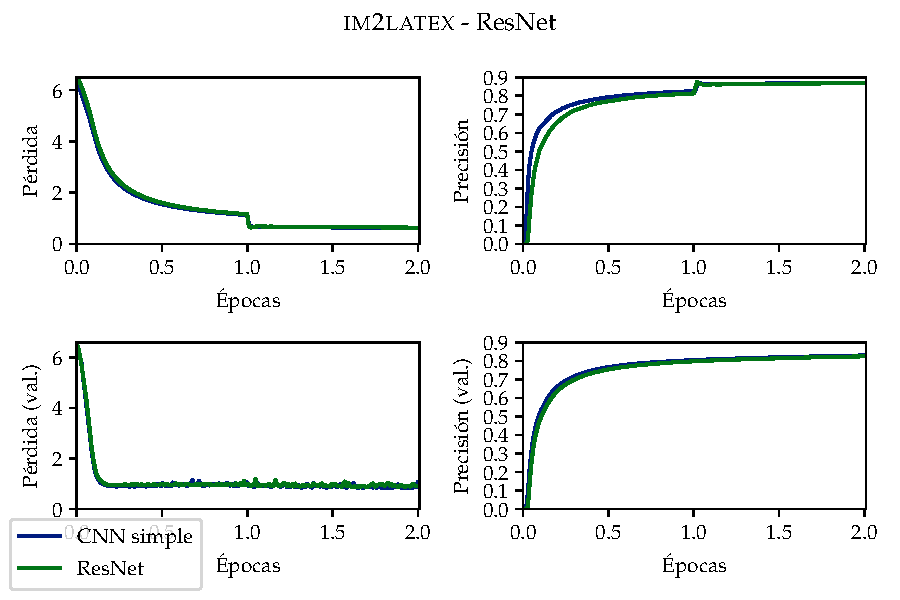
\includegraphics{fig/im2latex-3b.pdf}
\end{figure}

Observamos como el resultado de este modelo utilizando ResNet es ligeramente peor en
precisión que el modelo anterior. Sin embargo, la diferencia es realmente pequeña, y
es mayor en entrenamiento que en validación. De hecho, observando las gráficas de
precisión vemos como se reduce la precisión entrenamiento es considerablemente peor
durante la primera mitad de la primera epoch, mientra que la precisión en validación
es practicamente idéntica. Esto muestra como el modelo con ResNet se sobreajusta menos
manteniendo la misma precisión en validación. 

Estos resultados distan mucho de lo que esperábamos. Sustituir la CNN utilizada para
extraer las características de la imagen por una mejor debería repercutir positivamente
en los resultados del modelo.

Por otro lado, el tiempo de ejecución se reduce ligeramente. Es por ello que utilizaremos
ResNet en los experimentos finales.


\subsubsection{Codificación posicional 2-dimensional}
\label{exp:3c}

A continuación ponemos a prueba la codificación posicional 2-dimensional explicada en
esta sección \ref{feature:cod-pos-2d}. Para ello volvemos al modelo con una CNN simple
quitando ambigüedades, y le añadimos la codificación posicional 2-dimensional. Veamos
los resultados obtenidos:

\begin{table}[H]
	\centering
	\begin{tabular}{llllll}
		& Precisión       & Precisión en validación & Pérdida         & Pérdida en validación & Tiempo (h)    \\ \cline{2-6} 
		CNN Elim. Amb.   & \textbf{0.8701} & \textbf{0.8295}         & \textbf{0.6272} & \textbf{0.8406}       & 8.77          \\
		CNN Cod. Pos. 2d & 0.8151          & 0.7791                  & 1.2356          & 1.0639                & \textbf{3.60}
	\end{tabular}
\end{table}

\begin{figure}[H]
	\centering
	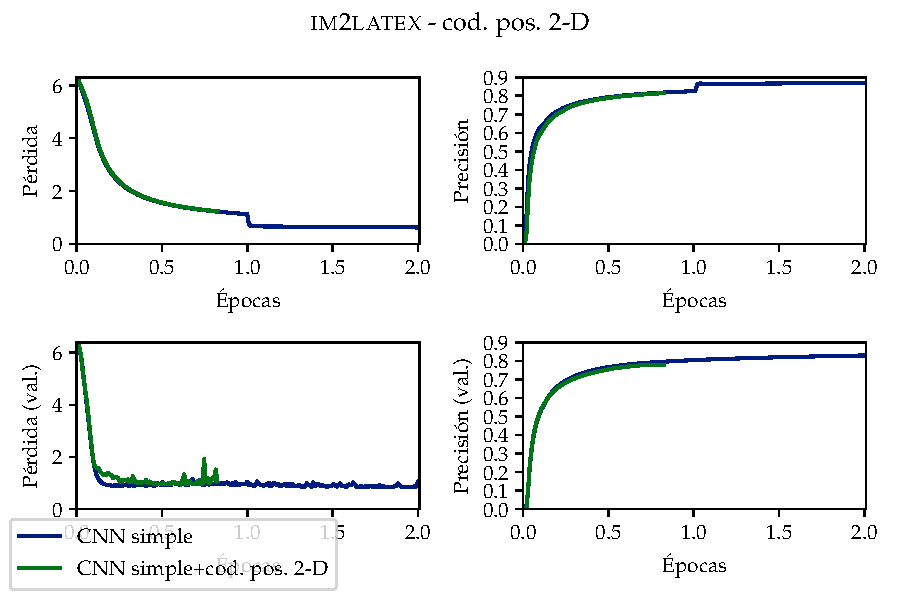
\includegraphics{fig/im2latex-3c.pdf}
\end{figure}

Como podemos ver, el \emph{early stopping} ha vuelto a activarse ante la falta de
convergencia. Aunque los resultados en precisión apenas varían, la evolución se ha
estancado antes de terminar la primera epoch. Los valores de pérdida en validación
si tardan más en converger y oscilan, aunque ya hemos observado oscilaciones
parecidas en experimentos anteriores.

En principio, este experimento no revela nada particularmente esclarecedor sobre la
codificación posicional 2-dimensional, solamente un estancamiento prematuro. Lo
utilizaremos en experimentos posteriores debido a esta inconclusión que debería
ser estudiada con mayor profundidad. 


\subsubsection{Learning rate modificado}

Este experimento es un poco distinto. No es de los experimentos que inicialmente
enfocamos como para poner en esta memoria, sino como uno utilizado para probar
distintas alternativas o ideas que quizas podrían mejorar el modelo pero no han
acabado funcionando. Es por ello que no hemos realizado más experimentos en esta
dirección. Sin embargo, creemos que por la idea merece la pena que destacarlo aquí.

El eje central de este experimento es la evolución del \emph{learning rate} del
modelo, originalmente es la siguiente:

\begin{figure}[H]
	\centering
	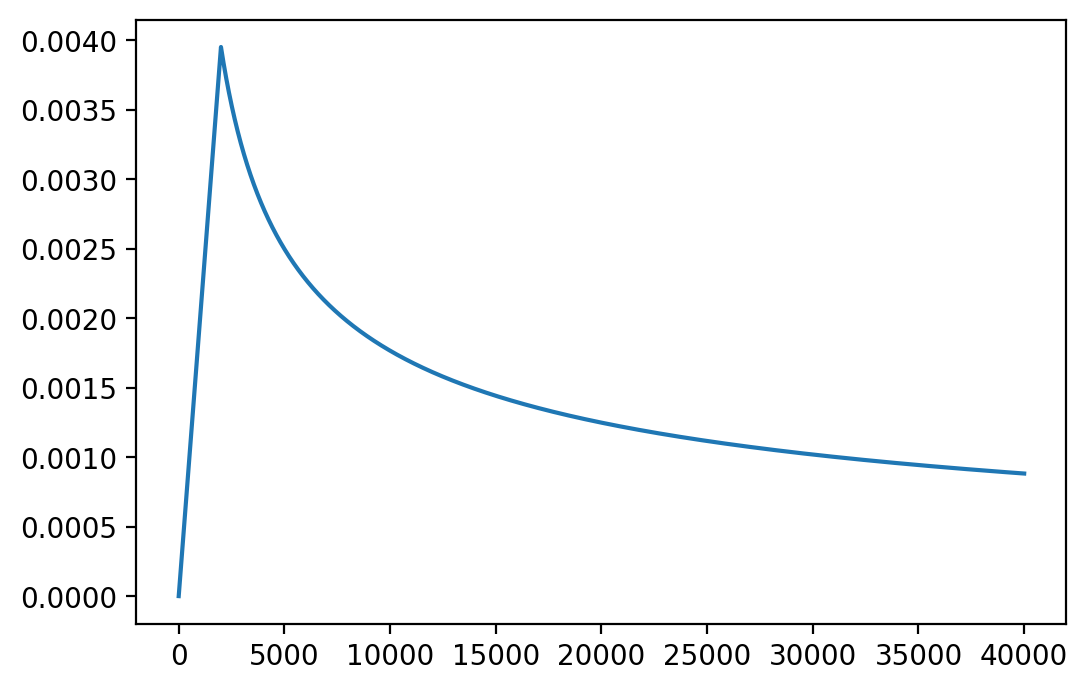
\includegraphics[scale=0.5]{fig/learning-rate}
	\caption{Evolución del learning rate original}
\end{figure}

Donde vemos el valor del \emph{learning rate} respecto al número de imágenes que
estudia el modelo. El \emph{learning rate} se inicializa a 0.0040 y se reduce poco
a poco conforme evoluciona el modelo. Nuestra idea fue permitir valores altos de
learning rate en ciertos puntos del modelo más desarollado. Esto permitiría al
modelo escapar de mínimos locales, siguiendo la terminología del \emph{Gradient
	Descent}. Propusimos la siguiente curva alterada:

\begin{figure}[H]
	\centering
	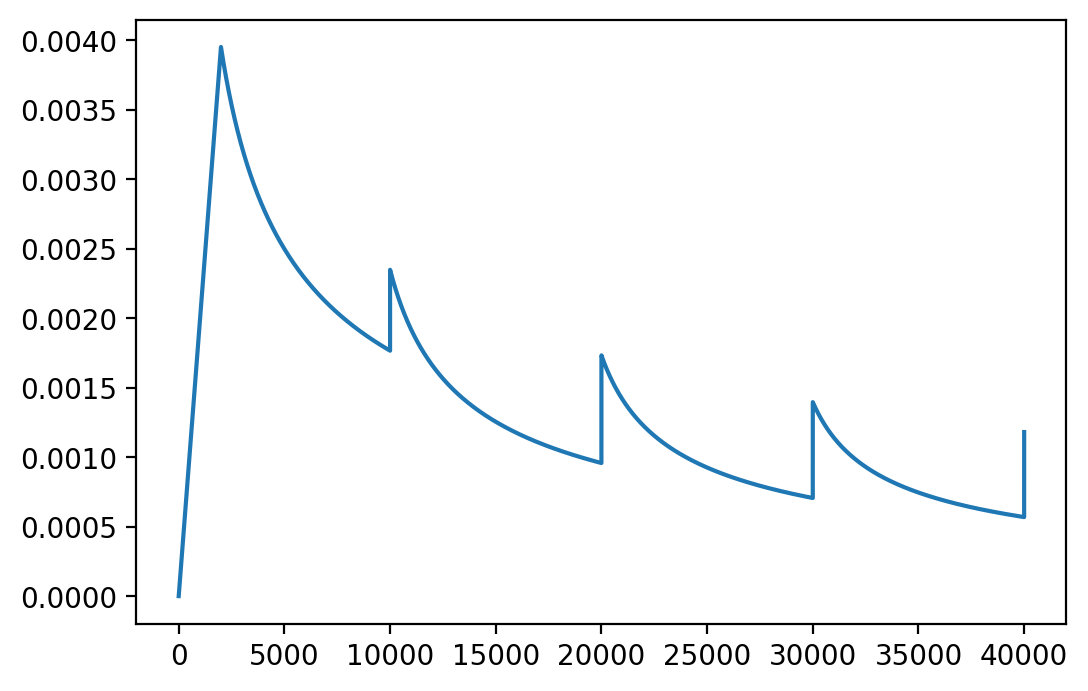
\includegraphics[scale=0.5]{fig/learning-rate2}
	\caption{Evolución del learning rate propuesto}
\end{figure}

Utilizando esta nueva evolución para el \emph{learning rate} lanzamos un nuevo
experimento. El modelo de este experimento es una combinación de los experimentos
\ref{exp:3a} y \ref{exp:3b}. Es decir, utiliza ResNet en vez de la CNN simple
utilizada en el modelo inicial junto con atención eficiente. Veamos los resultados
obtenidos:

\begin{table}[H]
	\centering
	\begin{tabular}{llllll}
		& Precisión       & Precisión en validación & Pérdida         & Pérdida en validación & Tiempo (h) \\ \cline{2-6} 
		CNN Elim. Amb.     & \textbf{0.8701} & \textbf{0.8295}         & \textbf{0.6272} & \textbf{0.8406}       & 8.77       \\
		Modelo Alternativo & 0.7956          & 0.7860                  & 1.4274          & 0.9771                & 2.70      
	\end{tabular}
\end{table}

\begin{figure}[H]
	\centering
	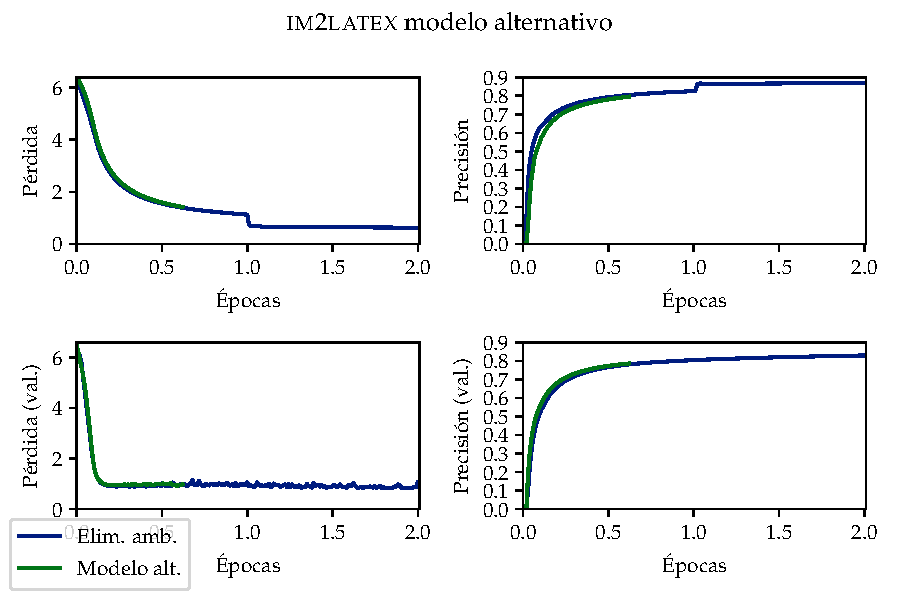
\includegraphics{fig/im2latex-alternativo.pdf}
\end{figure}

Como podemos ver, el modelo activó el \emph{early stopping} y se estanco mucho antes
que el resto de modelos estudiados hasta ahora. Es por ello que descartamos esta línea
de estudio.


\subsection{Experimentos finales}

Para estos ultimos experimentos buscamos obtener el mejor modelo posible en términos
de precisión en validación. Finalmente, evaluaremos el modelo correspondiente sobre el
conjunto de test.

\subsubsection{Combinación de los experimentos anteriores: Big boy}

En primer lugar combinaremos todas las características implementadas en todos los
experimentos anteriores y dejaremos que el modelo entrene todo lo posible sin alterar
nada más. En particular, Utilizaremos eliminación de ambigüedades (\ref{exp:2}),
atención eficiente (\ref{exp:3a}), ResNet en lugar de la red convolucional simple
(\ref{exp:3b}) y codificación posicional 2-dimensional (\ref{exp:3c}). 

Reconfiguramos el \emph{early stopping} para que sea active tras 10 evaluaciones
sin una mejora del 0.01\% de precisión en validación y entrenamos el modelo
durante 5 epochs. Veamos los resultados obtenidos:

\begin{table}[H]
	\centering
	\begin{tabular}{llllll}
		& Precisión & Precisión en validación & Pérdida & Pérdida en validación & Tiempo (h) \\ \cline{2-6} 
		Big Boy & 0.8889    & 0.8514                  & 0.5196  & 0.8602                & 20.23     
	\end{tabular}
\end{table}

\begin{figure}[H]
	\centering
	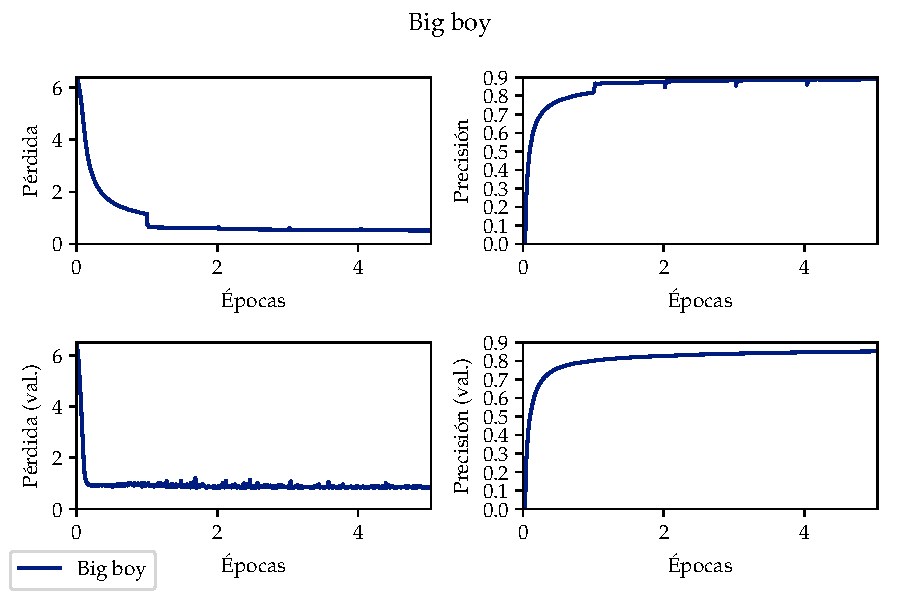
\includegraphics{fig/bigboy.pdf}
\end{figure}

Hemos obtenido una precisión del 85.14\% en validación, la mayor hasta ahora. Vemos como la evolución de la misma se produce sobretodo durante la primera epoch, como ya ocurría en los experimentos anteriores. Sin embargo, el modelo nunca llega a estancarse ya que no ha activado el \emph{early stopping} y ejecuta las 5 epochs al completo. Esto sugiere que podría mejorarse aún más, aunque sea ínfimamente, entrenándolo aún más.

Esto, claramente, no es una opción después de las 20.23 horas de entrenamiento que ha supuesto este experimento. Procedemos ahora a jugar con los parámetros del modelo para intentar mejorarlo todavía más.

\subsubsection{Bigger boy}

Para este último experimento antes de la evaluación final mantendremos el modelo anterior y reajustaremos algunos de sus parámetros. En particular:

% TODO: Dani si quieres dar mas informacion sobre estos parámetros y por qué, creo que peude venir bien

\begin{itemize}
	\item Aumentamos la profundidad del modelo de 20 a 32.
	\item Aumentamos el número de capas de 1 a 4.
	\item Aumentamos el número de cabezas de atención de 1 a 4, utilizando así atención multidimensional.
\end{itemize}

Adicionalmente, mantenemos la configuración de \emph{early stopping} pero reducimos el número de epochs a 3 para reducir el tiempo de cómputo total. Veamos los resultados obtenidos:

\begin{table}[H]
	\centering
	\begin{tabular}{llllll}
		& Precisión & Precisión en validación & Pérdida & Pérdida en validación & Tiempo (h) \\ \cline{2-6} 
		Big Boy    & 0.8889    & 0.8514                  & 0.5196  & 0.8602                & 20.23 \\
		Bigger Boy & 0.9054    & 0.8596                  & 0.4309  & 0.5976                & 18.40
	\end{tabular}
\end{table}

\begin{figure}[H]
	\centering
	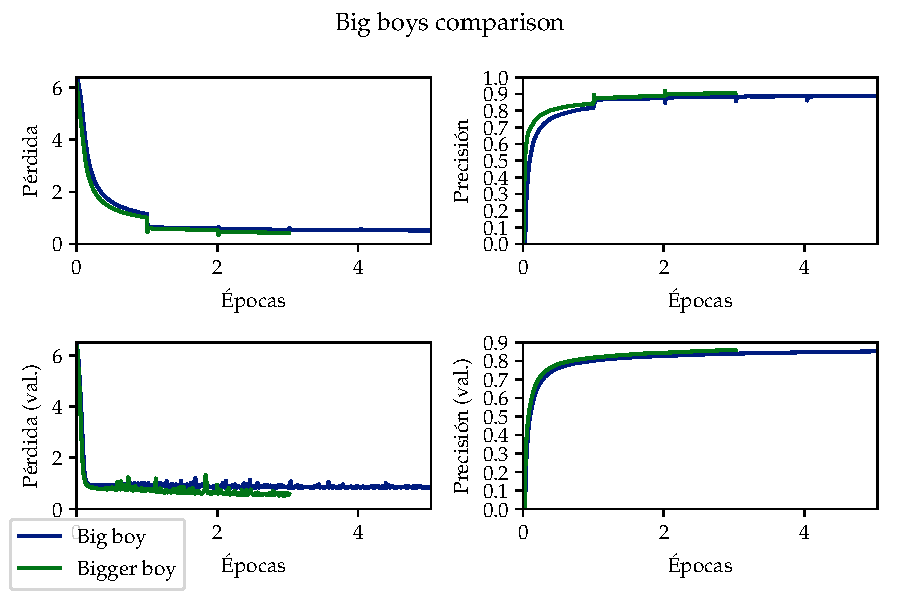
\includegraphics{fig/bigboys.pdf}
\end{figure}

Obteniendo en unicamente 3 epochs una precisión del 85.96\% en validación. Además, como se puede apreciar en las gráficas, las precisión en validación sigue creciendo cuando paramos el entrenamiento por encima de la del experimento anterior, volviendo a sugerir la necesidad de un entrenamiento prolongado.

Sin embargo, esta modificación en los parámetros nos ha salido cara: el tiempo de cómputo de 3 epochs ha aumentado a 18.40 horas. Esto nos indica que a pesar de que el tiempo sea cercano al de Big Boy, hemos conseguido mejor resultado con unicamente 3 epochs. Esto vuelve a reforzar la hipótesis de que con más datos el modelo sería aún mejor.

Cabe destacar finalmente la mejora en pérdida en validación. Esta es la primera comparación en la que puede observarse una mejora notable en este valor.


\subsubsection{Evaluación sobre test}

\section{Conclusiones}


\subsection{Trabajo futuro}

En esta sección exponemos las líneas de trabajo que no hemos podido explorar
por falta de tiempo:

\begin{itemize}
\item
	Aumento de datos: Hemos visto en distintos experimentos como no son
	necesarias muchas epochs sobre los mismos datos, sino más datos distintos
	entre sí. De cara a generar nuevos datos se puede generar una gramática más
	compleja que la creada para la base de datos sintética, o bien aplicar
	técnicas de visión por computador a las imágenes, aunque con muchas
	restricciones para no invalidar los resultados asociados.
	
\item
	En el experimento \ref{exp:3b} vimos como sustituir la CNN simple utilizada
	por una ResNet no mejoraba particularmente los resultados. La extracción
	de características es un proceso fundamental de nuestro modelo y deberíamos
	estudiar cómo mejorar el modelo en ese sentido. Quizás una red CNN simple
	sea suficiente para obtener toda la información de imágenes relativamente
	sencillas como las que utilizamos. Sería necesario estudiar un equilibrio
	entre buena extracción de características y minimizar el tiempo de ejecución
	en esta sección del modelo.
	
\item
	En el experimento \ref{exp:3c} estudiamos la codificación posicional
	2-dimensional sin llegar a ninguna conclusión específica. Actualmente
	no estamos seguros de si mejora o empeora el modelo, sólo de que las
	variaciones en los resultados obtenidas al introducir esta característica
	en el modelo no son especialmente agresivas. Sería necesario estudiar en
	profundidad esta modificación.
\end{itemize}

%%%%%%%%%%%%%%%%%%%%%%%%%%%%%%%%%%%%%%%%%%%%%%%%%%%%%%%%%%%%%%%%%%%%%%%%%%%%%%%%

\printbibliography

\end{document}
